% !TEX encoding = IsoLatin

% La riga soprastante serve per configurare gli editor TeXShop, TeXWorks
% e TeXstudio per gestire questo file con la codifica IsoLatin o Latin 1
% o ISO 8859-1.

% per commentare una riga mettere % al suo inizio
% per s-commentare una riga (ossia attivarla) togliere il % al suo inizio
%
\documentclass[pdfa% formato PDF/A, obbligatorio per l'archiviazione delle tesi di Polito
,cucitura%lascia margine per la rilegatura
%,twoside% per stampa fronte-retro (fortemente consigliato per tesi voluminose, opzionale per le altre)
%,12pt% font pi� grande (12pt) rispetto a quello normalmente usato (11pt)
]{toptesi}
%
\usepackage{hyperref}
\hypersetup{%
    pdfpagemode={UseOutlines},
    bookmarksopen,
    pdfstartview={FitH},
    colorlinks,
    linkcolor={blue},
    citecolor={red},
    urlcolor={blue}
  }
% \documentclass[11pt,twoside,oldstyle,autoretitolo,classica,greek]{toptesi}
% \usepackage[or]{teubner}
%%%%%%%%%%%%%%%%%%%%%%%%%%%%%%%%%%%%%%%%%%%%%%%%%%%%
%
% Esempio di composizione di tesi di laurea.
%
% Questo esempio e' stato preparato inizialmente 13-marzo-1989
% e poi e' stato modificato via via che TOPtesi andava
% arricchendosi di altre possibilita'.
%
% Nel seguito laurea "quinquennale" sta anche per "specialistica" o "magistrale"

% Cambiare encoding a piacere; oppure non caricare nessun encoding se si usano
% solo caratteri a 7 bit (ASCII) nei file d'entrata.
%
\usepackage[latin1]{inputenc}% IMPORTANTE! usare codifica ISO-8859-1 per le lettere accentate

% !TEX encoding = IsoLatin

% per inserire uno spazio "fantasma" nella definizione di un'abbreviazione
\usepackage{xspace}

% per inserire un DOI senza problemi coi caratteri "strani" ivi presenti
\usepackage{doi}
\renewcommand{\doitext}{DOI }% originally was "doi:"

% per inserire correttamente le unit� di misura SI (incluse quelle binarie)
\usepackage[binary-units]{siunitx}
% se si desidera usare / invece che la potenza -1 per indicare "al secondo"
\sisetup{per-mode=symbol}

% per inserire codice di programmazione complesso
\usepackage{listings}% per inserire codice di programmazione complesso
\lstset{
basicstyle=\ttfamily,
columns=fullflexible,
xleftmargin=3ex,
breaklines,
breakatwhitespace,
escapechar=`
}

% modify some page parameters
\setlength{\parskip}{\medskipamount}

% riga orizzontale
\newcommand{\HRule}{\rule{\linewidth}{0.2mm}}
% esempio di creazione di semplici abbreviazioni
\newcommand{\ltx}{\LaTeX\xspace}
\newcommand{\txw}{TeXworks\xspace}
\newcommand{\mik}{MikTex\xspace}
\newcommand{\html}{HTML\xspace}
\newcommand{\xhtml}{XHTML\xspace}

% esempio di creazione di un'abbreviazione con un parametro (il cui uso � indicato da #1)
\newcommand{\cmd}[1]{\texttt{#1}\xspace}
% per citare un RFC, es. \rfc{822}
\newcommand{\rfc}[1]{RFC-#1\xspace}
% per citare un file (es. \file{autoexec.bat}) o una URI fittizia (es. \file{http://www.lioy.it/})
% per le URI vere usare \url o \href
\newcommand{\file}[1]{\texttt{#1}\xspace}
% per inserire codice di esempio in-line
\newcommand{\code}[1]{\lstinline|#1|}
% importante per i pathname Windows perch� non si pu� usare \ essendo un carattere riservato di Latex
\newcommand{\bs}{\textbackslash}
% definizione di un termine: formattazione ed inserimento nell'indice
\newcommand{\tdef}[1]{\textit{#1}\index{#1}}
% meta-termine, usato tipicamente nelle definizioni dei tag
\newcommand{\meta}[1]{\textit{#1}}
% abbreviazioni in inglese
\newcommand{\ie}{i.e.\xspace}
\newcommand{\eg}{e.g.\xspace}

\begin{document}
	
\selectlanguage{english}

\ateneo{Politecnico di Torino}

%%% scegliere la propria facolt� (solo PRIMA dell'AA 2012-2013)
%
%\facolta[III]{Ingegneria dell'Informazione}
%\facolta[IV]{Organizzazione d'Impresa\\e Ingegneria Gestionale}
%\Materia{Remote sensing}% uso sconsigliato

%\monografia{Gestione informatizzata di un magazzino ricambi}% per la laurea triennale
\titolo{Automatic Malware Signature Generation}% per la laurea quinquennale e il dottorato
%\sottotitolo{Metodo dei satelliti medicei}% NON obbligatorio, per la laurea quinquennale e il dottorato

%%% scegliere il proprio corso
%
%\corsodilaurea{Ingegneria dell'Organizzazione d'Impresa}% per la laurea di primo e secondo livello
%\corsodilaurea{Ingegneria Logistica e della Produzione}% per la laurea di primo e secondo livello
%\corsodilaurea{Ingegneria Gestionale}% per la laurea di primo e secondo livello
\corsodilaurea{Ingegneria Informatica}% per la laurea di primo e secondo livello
%\corsodidottorato{Meccanica}% per il dottorato

\candidato{Michele \textsc{Crepaldi}}% per tutti i percorsi
%\secondocandidato{Evangelista \textsc{Torricelli}}% per la laurea magistrale solamente
%\direttore{prof. Albert Einstein}% per il dottorato
%\coordinatore{prof. Albert Einstein}% per il dottorato
\relatore{prof.\ Antonio Lioy}% per la laurea e il dottorato
\secondorelatore{ing.~Andrea Atzeni}% per la laurea magistrale
%\terzorelatore{{\tabular{@{}l}dott.\ Neil Armstrong\\prof. Maria Rossi\endtabular}}% per la laurea magistrale
%\tutore{ing.~Andrea Atzeni}% per il dottorato
%\tutoreaziendale{dott.\ ing.\ Giovanni Giacosa} % solo per la laurea di secondo livello con tesi svolta in azienda
%\NomeTutoreAziendale{Supervisore aziendale\\Centro Ricerche FIAT}
%\sedutadilaurea{Agosto 1615}% per la laurea quinquennale
%\esamedidottorato{Novembre 1610}% per il dottorato
%\sedutadilaurea{\textsc{Novembre} 2017}% per la laurea triennale
\sedutadilaurea{\textsc{Anno~accademico} 2020-2021}% per la laurea magistrale
%\annoaccademico{1615-1616}% solo con l'opzione classica
%\annoaccademico{2006-2007}% idem
%\ciclodidottorato{XV}% per il dottorato
\logosede{logopolito}
%
%\chapterbib %solo per vedere che cosa succede; e' preferibile comporre una sola bibliografia
%\AdvisorName{Supervisors}
%\newtheorem{osservazione}{Osservazione}% Standard LaTeX

%\usepackage[a-1b]{pdfx}
%\hypersetup{%
%    pdfpagemode={UseOutlines},
%    bookmarksopen,
%    pdfstartview={FitH},
%    colorlinks,
%    linkcolor={blue},
%    citecolor={green},
%    urlcolor={blue}
%  }

%
% per numerare e far comparire nell'indice anche le sezioni di quarto livello
% SCONSIGLIATO! da usarsi solo in caso di estrema necessit�
%\setcounter{secnumdepth}{4}% section-numbering-depth
%\setcounter{tocdepth}{4}% TOC-numbering-depth (TOC=Table-Of-Content)

%\setbindingcorrection{3mm}

\errorcontextlines=9

\frontespizio
\paginavuota
\newpage
%per sfruttare meglio lo spazio nella pagina
\advance\voffset -5mm
\advance\textheight 30mm

% opzionale, solo se si vuole dedicare la tesi a delle persone care
\begin{dedica}
A mio padre

\textdagger\ A mio nonno Pino
\end{dedica}

\sommario

Inserire qui un breve sommario della tesi.

\ringraziamenti

Opzionali, solo nel caso si sia ricevuto un aiuto speciale e particolarmente rilevante.

%% inserire sempre nella tesi per la laurea di I livello, perch� il nome dei tutori non � indicato sul frontespizio.
%Il lavoro descritto in questa monografia � stato svolto sotto la supervisione
%del Prof. Antonio Lioy (tutore accademico)% inserire sempre il nome del tutore accademico
% e dell'Ing. Mario Rossi (tutore aziendale)% inserire solo se la monografia � relativa ad un tirocinio.
%.

%\tablespagetrue % normalmente questa riga non serve ed e' commentata
%\figurespagetrue % normalmente questa riga non serve ed e' commentata

\indici

\mainmatter

\chapter{Scrivere testi complessi}

% !TEX encoding = IsoLatin

\section{Scrittura di un capitolo}

Dividere la tesi in capitoli (col comando \cmd{\bs chapter}) ed il capitolo in parti logiche mediante gli appositi comandi (\cmd{\bs section}, \cmd{\bs subsection} e \cmd{\bs subsubsection}).

Cercare inoltre di scrivere in  buon italiano perch� la tesi � un documento formale che viene archiviato per lungo tempo e costituisce parte della carriera di uno studente.

Questo capitolo di esempio contiene informazioni circa l'uso del sistema \ltx per la scrittura di testi scientifici (molto utile anche per la composizione della tesi di laurea).
Si consiglia di non limitarsi solo a leggere questo testo ma di esaminare il file \file{.tex}  corrispondente per imparare rapidamente i comandi \ltx tramite gli esempi contenuti in tale file sorgente.

\section{Installazione di un sistema \ltx}

Esistono tanti sistemi per elaborare testi scritti in \ltx. Per sistemi Windows si consiglia l'uso di \mik, che pu� essere scaricato dal seguente sito:

\url{http://www.miktex.org/}

\mik installa automaticamente anche \txw, un IDE (Integrated Development Environment) per \ltx che permette di scrivere il sorgente ed ottenere velocemente il PDF corrispondente, che viene mostrato in una finestra separata. \txw � integrato con un correttore ortografico ed � dotato di auto-completamento delle parole (ad esempio scrivendo \cmd{bit} e premendo quindi TAB viene generato automaticamente l'ambiente \cmd{itemize} per inserire una lista non ordinata); si veda la sezione 6.3 del \href{http://www.leliseron.org/texworks/}{manuale} di \txw per un elenco completo.
Notare anche che facendo click col tasto destro nella finestra che visualizza il PDF � possibile saltare automaticamente al punto corrispondente nella finestra di edit e viceversa.

\section{Convenzioni sui nomi dei file}

Poich� i diversi sistemi operativi hanno regole diverse circa i caratteri ammessi nei nomi dei file, per portabilit� nei diversi ambienti operativi � bene che tutti i file che compongono la tesi usino un sosttoinsieme di caratteri.
In particolare si suggerisce di usare solo caratteri alfanumerici  ed il carattere di sottolineatura, iniziando sempre il nome del file con un carattere che sia alfabetico o la sottolineatura.

%%%%%%%%%%

\section{Comporre testi con \ltx}

In questa sezione vengono fornite alcune informazioni generali sull'uso del linguaggio \ltx per comporre testi complessi.

%%%%%%%%%%

\subsection{Testo normale}

Le lettere accentate\index{accenti} si possono scrivere direttamente (mediante i tasti presenti sulla propria tastiera) se si � specificata la codifica ISO-8859-1 in \mik:
\begin{verbatim}
  Edit > Preferences > Editor > Encoding > ISO-8859-1
\end{verbatim}
Altrimenti si possono usare le sequenze di escape (attenzione a quella per la lettera i accentata):
\`a, \`e, \'e, \`{\i}, \`o, \`u.

Si ricordi che in Italiano l'accento � quasi sempre grave. L'accento acuto si usa in pochi casi specifici, quali le parole perch�, poich� e finch�, o la coppia n� \ldots n�.

I segni di interpunzione devono essere attaccati alla parola che li precede e separati con uno spazio dalla parola che li segue:
\begin{quote}
(giusto) ``caspita, che bella notizia!''
\\
(sbagliato) ``caspita , che bella notizia!''
\\
(sbagliato) ``caspita ,che bella notizia!''
\end{quote}

L'apostrofo\index{apostrofo} deve essere attaccato sia alla parola che lo procede sia a quella che lo segue:
\begin{quote}
(giusto) ``l'oro � un metallo prezioso''
\\
(sbagliato) ``l' oro � un metallo prezioso''
\\
(sbagliato) ``l 'oro � un metallo prezioso''
\\
(sbagliato) ``l ' oro � un metallo prezioso''
\end{quote}

Lasciando una riga vuota si genera automaticamente un nuovo paragrafo,\index{paragrafo} ossia si va a capo, si lascia un piccolo spazio verticale e si indenta la prima riga del paragrafo.
E' importante cercare di organizzare il proprio testo in paragrafi che contengano insieme di frasi correlate. Quando si cambia argomento, si inizia un nuovo paragrafo. Si puo considerare questo testo come un buon esempio di suddivisione in paragrafi.

L'uso del comando \cmd{\bs\bs} per forzare un ritorno a capo � fortemente deprecato. In sua vece bisogna usare il comando corrispondente all'effetto che si desidera ottenere: ad esempio, se � terminato un paragrafo basta lasciare una riga vuota, se si vuole creare un elenco basta usare uno dei comandi per la creazione di una lista.

Attenzione ai doppi apici \index{virgolette} che devono essere creati usando due volte il tipo di apice appropriato (aperto o chiuso), come nel seguente caso:
\begin{quote}
il film ``Il Ciclone'' � stato diretto ed interpretato da Leonardo Pieraccioni.
\end{quote}
Se alcune parole ricorrono frequentemente nel testo e sono scritte in un modo particolare allora conviene definire un'opportuna abbreviazione nel preambolo del file, ossia prima di \cmd{\bs begin\{document\}}. Come esempi si vedano in questo file le definizioni e l'uso delle abbreviazioni \cmd{\bs ltx} per generare la parola \ltx e \cmd{\bs cmd} per presentare in modo opportuno i comandi.

E' anche facile creare delle note\index{note} a pi� di pagina\footnote{\ldots ma vanno usate con parsimonia.} che vengono numerate automaticamente.

Non bisogna dimenticare di usare un correttore ortografico. Per installare il dizionario necessario scaricare dal sito \url{http://wiki.services.openoffice.org/wiki/Dictionaries} il file ZIP corrispondente alla lingua prescelta (nel caso sia la lingua Inglese installare il dizionario British e non American) e quindi estrarre tutti i file nella  cartella
\begin{center}
\cmd{C:\bs Program Files\bs MiKTeX 2.9\bs hunspell\bs dicts}
\end{center}
Il correttore si attiva quindi scegliendo il men�:
\begin{verbatim}
  Edit > Spelling > lingua_desiderata
\end{verbatim}
Le parole errate compariranno evidenziate con una sottolineatura in rosso: sar� cos� possibile modificarle direttamente oppure -- cliccandoci sopra col tasto destro -- scegliere tra le opzioni di correzione proposte.

E' possibile scrivere parti della tesi in lingue diverse, specificando il linguaggio usato (importante in modo che il programma vada a capo in modo corretto). Segue una citazione in inglese:
\selectlanguage{english}
\begin{quotation}
The man in the rubber boots and a thick coat to protect against the evening chill walked purposefully about a farm here, scattering pheasants as he went. He could have been an English gentleman out for a bit of hunting, except he carried no gun.

In his current circumstance, the WikiLeaks founder Julian Assange is more hunted than hunter, fighting extradition to Sweden on accusations of sexual misconduct while struggling to maintain the influence of WikiLeaks even as he remains here at Ellingham Hall, the country manor house of Vaughan Smith, a former soldier and journalist who runs a restaurant and club for journalists in London. 
\end{quotation}
\selectlanguage{italian}
Adesso si riprende il normale testo in Italiano, che seguir� le regole di composizione della lingua Italiana.

\index{citazioni!testuali}
Per inserire citazioni testuali (ossia porzioni di testo) si pu� usare l'ambiente \cmd{quote} (citazione breve) oppure quello \cmd{quotation} (per citazioni lunghe, che posso essere composte da pi� paragrafi), come appena fatto qui sopra per la citazione in inglese.

\index{URL}
Per inserire collegamenti a pagine o documenti web si usano i comandi \cmd{\bs url} e \cmd{\bs href} del package \file{hyperref} come nei due esempi seguenti:
\begin{description}
\item[uso di \cmd{\bs href}]\mbox{}\\
(sorgente) \verb+Nel \href{http://www.polito.it/}{sito web} del Politecnico di Torino+
\\
(risultato) Nel \href{http://www.polito.it/}{sito web} del Politecnico di Torino
\item[uso di \cmd{\bs url}]\mbox{}\\
(sorgente) \verb+Il sito web del Politecnico di Torino � \url{http://www.polito.it/}+
\\
(risultato) Il sito web del Politecnico di Torino � \url{http://www.polito.it/}
\end{description}

\index{citazioni!bibliografiche}
Infine � possibile citare testi o siti che sono stati consultati per la tesi: articoli a congresso \cite{psisec}, articoli su rivista \cite{tpa}, capitoli di libri \cite{tc}, siti o pagine web \cite{openssl} e RFC (come \rfc{5246} \cite{tls12} che definisce la versione 1.2 del protocollo TLS).
Si noti che le voci della bibliografia devono essere elencate nell'apposita sezione (comando \cmd{\bs thebibliography}) secondo l'ordine in cui vengono citate.
Per bibliografie pi� complesse � possibile l'uso di BibTex, ma � sconsigliato se non si supera la decina di citazioni.
Per ulteriori informazioni si veda la Sez.~\ref{sec:bibliografia}.

%%%%%%%%%%

\subsection{Liste}

\index{liste!non ordinate}
Usare liste puntate per elenchi in cui l'ordine non � importante, come nel caso degli esami obbligatori da superare per essere ammessi al secondo anno:
\begin{itemize}
\item
Analisi Matematica I;
\item
Fisica I;
\item
un esame a scelta tra Chimica ed Informatica.
\end{itemize}
Notare che normalmente ogni elemento della lista � costituito da un'unica frase, terminata da punto-e-virgola, tranne l'ultimo elemento che � terminato da un punto. Ogni punto inizia con lettera minuscola (a meno che la parola iniziale sia un sigla o un nome proprio). E' fortemente sconsigliato l'uso di una lista se uno o pi� punti contengono pi� di una singola frase. In questo caso conviene scrivere paragrafi separati oppure creare delle sottosezioni.

\index{liste!ordinate}
Le liste numerate si creano con l'ambiente \cmd{enumerate} e sono utili per elencare elementi aventi un ordine di priorit�, come nel caso della ricetta per cucinare la pastasciutta:
\begin{enumerate}
\item
prendere una pentola;
\item
riempirla di acqua;
\item
metterla sul fuoco e portare l'acqua ad ebollizione;
\item
quando l'acqua bolle, buttare la pasta;
\item
quando la pasta � cotta, scolarla, condirla e \ldots mangiarla!
\end{enumerate}
\index{liste!di descrizioni}
Si possono anche fare delle liste che servono per descrivere generici oggetti, usando l'ambiente \cmd{description}.
L'oggetto descritto viene automaticamente posizionato ad inizio riga e scritto in grassetto, come nel seguente esempio:
\begin{description}
\item[pentola]
oggetto metallico usato per cuocere cibi;
\item[mela]
frutto che fa molto bene alla salute;
\item[Sarchiapone] animale immaginario usato in una gag di Walter Chiari e poi ripreso in un programma radiofonico da Renzo Arbore.
\end{description}

%%%%%%%%%%

\subsection{Formule matematiche ed unit� di misura}

\index{formule matematiche}
Le formule matematiche si possono scrivere direttamente nel corpo del testo racchiudendole tra due simboli \verb+$+
(come in questo esempio per il calcolo della circonferenza, $c = 2 \pi r$)
oppure scrivere la formula su una riga centrata racchiudendola tra \verb+\[+ e \verb+\]+:
\[
c = 2 \pi r
\]
Apici, pedici, frazioni, puntini e sommatorie sono anche semplici da fare:
\[
k = a_0 + a_1 \frac{1}{x} + a_2 \frac{1}{x^2} + \dots = \sum_{i=0}^N a_i \frac{1}{x^i} = \sum_{i=0}^N a_i x^{-i}
\]
Ecco ora un esempio di limite:
\[
\lim_{x\to\infty}f(x)=0
\]
\index{unit� di misura}
Quando si usano delle grandezze fare attenzione alle unit� di misura: usare sempre il SI e scrivere correttamente i simboli (ad esempio, il simbolo del chilo � la lettera ``k'' minuscola non la ``K'' maiuscola).
Per evitare errori e lasciare il giusto spazio tra quantit� e simbolo si suggerisce l'uso del package \cmd{siunitx} che aggiunge i comandi \cmd{\bs si} per unit� isolate o \cmd{\bs SI} per quantit� numerica seguita dalla sua unit� di misura.
Ecco un esempio d'uso per citare unit� isolate:
\begin{quote}
\ldots fornire il risultato in \si{\square\centi\metre}.
\end{quote}
ma � anche possibile indicare l'unit� su quantit� numeriche specifiche, citate in-line (ad esempio, un sacco di patate da \SI{10}{\kilo\gram}) o all'interno di una formula matematica:
\[
v = \frac{s}{t} = \frac{ \SI{100}{\meter} }{ \SI{5}{\second} } = \SI{20}{\meter\per\second}
\]

Nel caso di unit� relative al sistema binario � possibile adottare sia la vecchia notazione, che usa gli stessi prefissi del SI ma sottointende l'uso delle potenze di 2, sia la nuova notazione, in cui i prefissi del sistema binario sotto caratterizzati da una ``i'' minuscola.
Ad esempio:
\[
\SI{1}{\tera\byte}\ \mbox{(vecchia notazione)} =
\SI{1}{\tebi\byte}\ \mbox{(nuova notazione)} =
2^{30} \si{\byte}
\]

%%%%%%%%%%

\subsection{Tabelle e figure}

\index{tabelle}
In \ltx le tabelle si compongono descrivendo le righe di cui sono composte:
\begin{center}
\begin{tabular}{|l|c|c|}% posizionamento del testo nelle colonne l:left c:center r:right
\hline
\textit{modello} & \textit{velocit�} & \textit{consumi} \\
                 & [ \si{km/h} ]          & [ l/\SI{100}{km} ] \\
\hline
Fiat 500 & 150 & 19 \\
Alfa Giulietta & 210 & 21.5 \\
Ferrari Testarossa & 320 & 5.7 \\
\hline
\end{tabular}
\end{center}
Normalmente � meglio non inserire le tabelle direttamente nel testo ma creare un oggetto separato, con una didascalia ed un numero per citarlo ove necessario. Ad esempio � stata creata in questo modo la tabella~\ref{tab:voti} che riporta i voti conseguiti in alcuni esami da un ipotetico studente ma � slegata da questo specifico paragrafo. In questo modo \ltx sistemer� la tabella in un punto opportuno del testo, evitando di lasciare spazio verticale inutilizzato.
Si noti l'uso del carattere ``tilde'' (\textasciitilde) per tenere legato il numero della tabella (o figura o altro elemento flottante) alla parola che lo precede.

\begin{table}[tbh] % per piazzare la tabella t:top b:bottom h:here in ordine di preferenza; h � sconsigliato
\begin{center}
\begin{tabular}{|l|c|c|}
\hline
\textit{esame} & \textit{data} & \textit{voto} \\
\hline
Analisi I & 27/1/2009 & 18 \\
Informatica & 14/2/2009 & 30 \\
Fisica I & 15/7/2009 & 27 \\
\hline
\end{tabular}
% \caption contiene il testo della didascalia: limitarsi ad un una sola riga
% notare l'uso di \label per creare un'etichetta per citare la figura tramite \ref
% N.B. quando ci sono label o indici bisogna sempre elaborare due volte il file latex perch� la prima crea i riferimenti e la seconda li inserisce
\caption{Voti riportati negli esami sinora sostenuti.\label{tab:voti}}
\end{center}
\end{table}

\index{figure}
Per quanto riguarda le figure, conviene disegnarle con un apposito programma (es. PowerPoint) e poi salvarle in un file che verr� richiamato nel file \ltx.
Si consiglia di prestare attenzione ai font usati (suggeriti Arial o Helvetica), alla dimensione (minimo \SI{10}{pt}) e di generare un formato grafico ad alta definizione (PDF � il preferito, altrimenti PNG o JPG ad alta qualit�).
Il file grafico verr� poi incluso in \ltx per generare la figura, come nell'esempio della figura~\ref{fig:popTorino} che riporta il grafico della variazione di popolazione della citt� di Torino.
Si noti che questo grafico � di bassa qualit� (pixel percepibili ad occhio nudo) perch� salvato come JPG a bassa risoluzione (solo \SI{96}{DPI}).
Per i formati raster si dovrebbe sempre usare una risoluzione di almeno \SI{300}{DPI}.
%
\begin{figure}[tbh]% per piazzare la tabella t:top b:bottom h:here, in ordine di preferenza; h � sconsigliato
\centerline{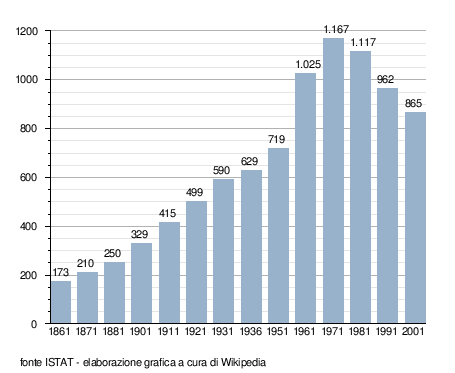
\includegraphics[width=0.9\textwidth]{torino.png}}
\caption{Popolazione di Torino, in migliaia di abitanti (fonte: \href{http://it.wikipedia.org/wiki/Torino}{wikipedia}).\label{fig:popTorino}}
\end{figure}
%
Nel caso che la figura non abbia gi� la dimensione desiderata si pu� ingrandirla o rimpicciolirla usando i parametri \cmd{width} (larghezza), \cmd{height} (altezza) o \cmd{scale}.
Quando si indica larghezza o altezza conviene farlo come una frazione della pagina; ad esempio per avere una figura che occupa il 90\% della larghezza pagina si scrive \cmd{width=0.9\bs textwidth} mentre si scrive \cmd{height=0.5\bs texteight} per una figura che deve occupare il 50\% dell'altezza della pagina.
Il parametro \cmd{scale} permette invece di indicare la dimensione come percentuale di quella originale della figura.
Ad esempio se la figura originale contiene testo con font a \SI{20}{pt} conviene scalarla al 50\% (in modo che la figura abbia font a \SI{10}{pt}) usando il parametro \cmd{scale=0.5}. L'uso di \cmd{scale} � fortemente consigliato nel caso che la figura contenga del testo, in modo da armonizzarne la dimensione con quello del corpo della pagina.

Se un'immagine � stata copiata da una fonte esterna, tale fonte deve essere indicata nella didascalia (come fatto ad esempio nella figura~\ref{fig:popTorino}).

\begin{figure}[tb]
\HRule
\begin{lstlisting}
#include <stdio.h>

int main ()
{
   printf ("Ciao!\n");
   return 0;
}
\end{lstlisting}
\HRule
\caption{Esempio di programma inserito tramite \cmd{lstlisting}.\label{fig:prog}}
\end{figure}
Nel caso che sia necessario includere del codice sorgente (cosa da fare con estrema parsimonia e solo in caso sia realmente necessario, ossia non includere codice solo per fare volume) si pu� usare l'ambiente \cmd{lstlisting} che include testo rispettandone la formattazione originale ed usando un font a spaziatura fissa, come nell'esempio in Fig.~\ref{fig:prog}.
E' anche possibile numerare le righe del programma, come nell'esempio in Fig.~\ref{fig:prog-num}, ma la numerazione � da usarsi solo se nel testo si deve far riferimento a specifiche sezioni del programma.

\begin{figure}[tb]
\HRule
\begin{lstlisting}[numbers=left]
#include <stdio.h>

int main ()
{
   printf ("Ciao!\n");
   return 0;
}
\end{lstlisting}
\HRule
\caption{Esempio di programma inserito tramite \cmd{lstlisting} con  numerazione delle righe.\label{fig:prog-num}}
\end{figure}

Per citare piccoli pezzi di codice si pu� usare direttamente l'ambiente \cmd{lstlisting} nel testo (invece che in una figura separata), come nel seguente esempio relativo al codice \html per centrare un testo:
\begin{lstlisting}
<center>
Esempio di testo centrato.
</center>
\end{lstlisting}
Quando invece si vuol citare del codice (molto corto) all'interno di una riga si pu� usare \cmd{\bs code} come in questo caso in cui dico che in \html per centrare del testo si pu� usare il tag \code{<center>} ma � deprecato (meglio usare uno stile CSS).

%%%%%

\section{La bibliografia\label{sec:bibliografia}}

Anche se siamo nell'era di Internet e dei motori di ricerca, � buona norma citare con precisione le fonti a cui si � attinto per scrivere la tesi. 

I nomi degli autori devono essere specificati con l'iniziale del nome, seguita da punto e quindi dal cognome.

Nel caso di articoli su rivista, deve essere indicato il titolo dell'articolo, il nome della rivista, il numero del fascicolo (solo se la rivista � numerata), il mese e l'anno di pubblicazione,  la pagina di inizio e fine dell'articolo.

Nel caso di articoli pubblicati a congresso, convegno o workshop, deve essere indicato il titolo dell'articolo, il nome del congresso, il luogo del congresso (citt� seguita dalla nazione tra parentesi tonde), la data e la pagina di inizio e fine dell'articolo.
Nel caso di citt� negli USA, occorre indicare anche lo stato, ad esempio ``Portland (OR, USA)''.

Nal caso di libri si indicano gli autori, il titolo del libro, l'editore e l'anno di pubblicazione. Se si vuole citare uno specifico capitolo o insieme di pagine, si inserisce tale indicazione nel testo del documento (come indicato pi� avanti) e non nella voce bibliografica.

Se si citano documenti pubblici (es. standard, RFC, report tecnici, pagine web) occorre fornire oltre ai dati identificativi anche la URL tramite cui � possibile accedere al documento.

Qualunque sia la tipologia di articolo, � molto importante citare -- se disponibile -- il \tdef{DOI} (Digital Object Identifier). Questo � un codice universale che identifica univocamente una pubblicazione, sia essa a stampa o in formato elettronico. Specificando il DOI come se fosse una pagina all'interno del sito \url{http://dx.doi.org/} si viene ridiretti automaticamente alla pubblicazione corrispondente. Normalmente tutte le pubblicazioni recenti e di qualit� hanno un DOI assegnato, mentre per quelle pi� vecchie o di minore qualit� il DOI � raramente disponibile.

Si veda la bibliografia presente in questo testo come esempio di corretta e completa citazione di vari tipi di riferimenti bibliografici.
Si noti che ogni elemento della bibliografia non � terminato dal carattere punto.

Le citazioni si inseriscono nel testo usando il comando \cmd{\bs cite} seguito in parentesi graffe dalla sigla usata per identificare il riferimento bibliografico.
Il comando \cmd{\bs cite} deve essere separato con uno spazio dalla parola che lo precede:
\begin{quote}
(giusto) \verb+il protocollo TLS \cite{tls12} � usato per la sicurezza del web+
\\
(sbagliato) \verb+il protocollo TLS\cite{tls12} � usato per la sicurezza del web+
\end{quote}
In questo esempio \cmd{tls12} � la sigla usata nella sezione della bibliografia come identificativo mnemonico dello standard TLS (per il dettaglio del formato bibliografico si veda il relativo sorgente nel file \file{biblio.tex}).

Quando si vuole citare una specifica parte di un riferimento bibliografico (es. una figura o un capitolo) si inserisce tra parentesi quadre (prima delle graffe) l'indicazione della specifica parte, come nel seguente esempio:
\begin{quote}
(sorgente) \verb+Il record protocol di TLS \cite[Sez.~5]{tls12} � usato per \ldots+
\\
(risultato) Il record protocol di TLS \cite[Sez.~5]{tls12} � usato per \ldots
\end{quote}

Se la bibliografia � corta (non pi� di dieci-venti voci bibliografiche) allora la si pu� comporre ``a mano'' usando l'ambiente \cmd{\bs thebibliography} ed indicando gli elementi della bibliografia tramite \cmd{\bs bibitem}.
Nel caso di bibliografie pi� complesse � consigliato l'uso di BibTeX usando il file di stile \file{torsec.bst}.

Si osservi che Wikipedia, ancorch� molto utile, non � una fonte attendibile in quanto il suo contenuto varia nel tempo e pu� non essere stato adeguatamente verificato.
Se ne sconsiglia quindi l'uso in una tesi di laurea.

%%%%%%%%%%

\section{Nomi dei file}
Tutti i nomi dei file che compongono la tesi (inclusi quelli di supporto, come figure e grafici) non devono contenere il carattere ``spazio'' in quanto tale carattere � permsso in alcuni filesystem (es. NTFS di Windows) ma causa problemi in altri (es. EXTFS di Linux).
Quindi per portabilit� se ne deve sempre evitare l'uso.

%%%%%%%%%%

\section{Conclusioni}

Queste sono solo delle brevi note sull'uso di \ltx per comporre semplici testi.
Per necessit� pi� complesse si conmsiglia di consultare leggere la documentazione che viene installata assieme a \ltx.
In particolare con \mik (versione 2.9) la documentazione viene installata nella cartella
\begin{center}
\file{C:\bs Program~Files\bs MiKTeX~2.9\bs doc}
\end{center}
ed in particolare quella relativa ai vari package nella sottocartella \file{latex\bs nome-del-package}; ad esempio, la documentazione del package \cmd{siunitx} si trova nella cartella
\begin{center}
\file{C:\bs Program~Files\bs MiKTeX~2.9\bs doc\bs latex\bs siunitx}
\end{center}
Inoltre � sempre possibile consultare l'ampia documentazione disponibile in rete.


\chapter{La tesi di laurea magistrale}

\section{Struttura della tesi}

Normalmente la tesi per la laurea magistrale � composta da almeno cinque capitoli.

Il primo capitolo contiene l'introduzione e descrive il contesto o il problema da cui � scaturito l'argomento della tesi.
In altre parole, fornisce una giustificazione per lo svolgimento della tesi e dovrebbe incuriosire il lettore a scoprire come il problema � stato affrontato e risolto.

Nel caso di una tesi svolta in azienda � possibile inserire anche una breve descrizione dell'azienda o ente presso cui � stata svolta, con particolare riferimento al contesto applicativo, ingegneristico o commerciale da cui � nata la necessit� alla base della tesi.

Il secondo capitolo fornisce -- se necessario -- un'analisi critica dei lavori precedenti sul tema trattato nella tesi.

Il terzo capitolo descrive l'approccio usato per risolvere il problema. Ad esempio, nel caso di progettazione di un'applicazione web, si possono fornire le specifiche delle singole pagine, il collegamento tra le varie pagine, la struttura del database e la logica pplicativa.
Questo capitolo pu� anche essere spezzato in pi� capitoli se dovesse risultare particolarmente voluminoso, dedicando ciascun capitolo ad uno specifico tema (es. la progettazione del database, la logica applicativa).

Il capitolo successivo fornisce i risultati dell'attivit� svolta, cercando di misurare i risultati in modo quantitativo.

Infine il capitolo conclusivo riassume i risultati conseguiti ed indica se ci sono ulteriori possibili sviluppi o miglioramenti.

\selectlanguage{english}
\section{Writing the thesis in English}

If the thesis is written in English, then some terms should be changed (such Capitolo that should become Chapter) and hyphenation should follow the rules of the English language.

To achieve this effect, please insert \verb+\selectlanguage{english}+ in the preamble
(that is, before \verb+\begin{document}+) and do not forget to select the UK-English dictionary for the spell checker.
\selectlanguage{italian}


\chapter{Progettazione}

Discutere in questo capitolo come � stata progettata la soluzione al problema trattato nella tesi, indicando anche se sono stati valutati vari possibili approcci o soluzioni pre-esistenti e giustificando le proprie scelte. Descrivere quindi la soluzione vera e propria.

Nel caso sia stato sviluppato del software non triviale, � buona norma dedicargli tre sezioni:
\begin{itemize}
\item architettura dell'applicazione (interazioni con gli utenti e con altri sistemi, moduli logici, flussi dati interni ed esterni);
\item manuale dello sviluppatore (descrizione dei moduli, degli algoritmi, delle interfacce e delle strutture dati);
\item manuale utente (come installare ed usare il programma, interfacce, comandi, dati in input ed in output).
\end{itemize}
Nel caso di software molto voluminoso, queste tre sezioni possono diventare tre capitoli separati.

\chapter{Risultati}

Inserire in questo capitolo i risultati conseguiti, cercando di analizzarli -- se possibile -- in modo quantitativo.


\chapter{Conclusioni}

Qui si inseriscono brevi conclusioni sul lavoro svolto, senza ripetere inutilmente il sommario.

Si possono evidenziare i punti di forza e quelli di debolezza, nonch� i possibili sviluppi futuri o attivit� da svolgere per migliorare i risultati.

% bibliografia scritta "a mano"
%% !TEX encoding = IsoLatin

% La bibliografia, da inserirsi solo se ci sono state citazioni.
% In questo caso ricordarsi che bisogna sempre elaborare due volte il file .TEX
% perch� la prima volta viene generata la bibliografia mentre la seconda volta viene inclusa

% NOTA: citare il DOI non � obbligatorio ma MOLTO desiderabile

\begin{thebibliography}{9} % se ci sono meno di 10 citazioni
%\begin{thebibliography}{99} % se ci sono da 10 a 99 citazioni
%\begin{thebibliography}{999} % se ci sono da 100 a 999 citazioni

% esempio citazione articolo a congresso
\bibitem{psisec}
% nomi autori
I.Enrici, M.Ancilli, A.Lioy,
% titolo articolo
``A psychological approach to information technology security'',
% nome del congresso
HSI-2010: 3rd Int. Conf. on Human System Interactions,
% luogo (stato) e data del congresso
Rzesz�w (Poland), May 13-15, 2010,
% pagine dell'articolo
pp.\ 459-466,
% DOI
\doi{10.1109/HSI.2010.5514528}

% esempio citazione articolo su rivista
\bibitem{tpa}
% autori dell'articolo
G.Cabiddu, E.Cesena, R.Sassu, D.Vernizzi, G.Ramunno, A.Lioy,
% titolo dell'articolo
``Trusted Platform Agent'',
% nome della rivista
IEEE Software,
% volume e numero della rivista (alcune riviste non ce l'hanno)
Vol.\ 28, No.\ 2,
% mese e anno di pubblicazione della rivista
March-April 2011,
% pagine dell'articolo
pp.\ 35-41,
% DOI
\doi{10.1109/MS.2010.160}


% esempio citazione capitolo di un libro fatto come collezione di contributi da autori diversi
\bibitem{tc}
A.Lioy, G.Ramunno, % autori del capitolo
``Trusted Computing'' % titolo del capitolo
nel libro % in the book
``Handbook of Information and Communication Security'' % titolo del libro
a cura di % edited by
P.Stavroulakis, M.Stamp, % nomi dei curatori
Springer, % nome editore
2010, % anno di pubblicazione
pp.\ 697-717, % pagine del capitolo
\doi{10.1007/978-3-642-04117-4_32}

 % esempio citazione pagina web di un progetto
\bibitem{openssl}
% nome del progetto
The OpenSSL project,
 % URI della pagina web
\url{http://www.openssl.org/}

% esempio citazione RFC
\bibitem{tls12}
T.Dierks, E.Rescorla,
``The Transport Layer Security (TLS) Protocol Version 1.2'',
\rfc{5246}, August 2008,
\doi{10.17487/RFC5246}

 % esempio citazione libro
\bibitem{seceng}
Ross J. Anderson,
``Security engineering'',
Wiley, 2008,
ISBN: 978-0-470-06852-6

\end{thebibliography}


% se la bibliografia � stata scritta (usando Bibtex) nel file biblio.bib allora commentare la riga precedente e scommentare le due righe seguenti
\bibliographystyle{torsec}
\bibliography{biblio}


\end{document}
